\section{Criteria to begin the LSST}

Armed with an understanding of the {\it as--built} system performance as outlined above and the Operations team readiness, we will use a set of objective criteria to gate the start of the LSST. These criteria will be concise and easily understandable so that the community of scientists, Rubin staff and other stakeholders counting on Rubin and the survey can have confidence the Observatory is on track.

The criteria articulated below are meant only to provide gating guidance signifying the survey start. There will be key processes within the overall system, including data management and processing where further work for improvements are required or desired after handover (beyond the construction project requirements). Unless these would prevent acquisition and saving of science quality data, thereby delaying the survey start, they are not discussed or enumerated here.  These and other criteria (TBD) will be used to gauge and monitor the overall performance of the Observatory and progress towards the 10--year survey objectives going forward, with nominal $T=0$ defined by when start criteria described herein are met.

The initial set of criteria developed by Operations team were discussed with the Science Advisory Committee and community at the 2024 Rubin Community Workshop. These criteria have evolved since that meeting and are presented here in the table below.

\begin{table}[]
\renewcommand{\arraystretch}{2}
\small
\centering
\caption{Survey Start Criteria}\label{tab:criteria}
\begin{tabular}{|p{0.25in}|p{1in}|p{4in}|p{1.0in}|}
\hline
Item & Criterion & Description& Status \\
\hline \hline

1 & \makecell[l]{LSSTCam\\ Maintenance} & Before the completion of SV, it is understood whether or not off TMA Camera maintenance will be needed within the first year of Operations.& \makecell[l]{No off TMA \\maintenance\\ required.}  \\\hline  

2 & SRD & All science requirements that can be verified with SV data are verified or expected to be verified within 3 months of completion of SV. & Check status at CCR3 \\\hline

3 & Dome & The dome environment is not limiting typical performance. &\makecell[l]{ Not controlled \\until after \\Handover} \\\hline

4 & Calibration & All necessary calibration data products are available at the time any LSST data are obtained or can be obtained after the fact without invalidating the observed data for inclusion in the LSST. & Check status at CCR3 \\\hline

5 & DIQ & The ''System'' contribution to the measured Delivered Image quality is better than or equal to 0.45$\arcsec$ & \makecell[l]{Currently 0.6$\arcsec$ \\system \\contribution}\\\hline

6 & Normalized \'{E}tendue (\it{eF}) & Survey Speed  is $>$ 0.7. & Currently 0.68 \\\hline

7 & Cadence & The scientific merits and technical feasibility of the planned survey scheduler algorithms for DR1 have bee reviewed and verified. & In progress\\\hline

8 & Early Science & DP2 observations are completed as planned \citep{RTN-011}.& \makecell[l]{SV is complete; \\a report will be delivered by \\October.} \\

\hline
\end{tabular}
\end{table}

The initial boundary conditions for determining the start criteria are that the construction project has successfully accomplished its own Construction Completeness Criteria (\cite{SITCOMTN-005}) and has passed the third Construction Completeness Review (CCR3).  Successful completion of CCR3 means NSF and DOE have accepted the system as the one that was intended to be built and will operate to conduct the 10-year LSST science program.  

The survey start criteria cover a range of contexts.  The criteria are not meant to be comprehensive with respect to gauging and monitoring LSST's scientific progress and success. They are intended to serve as a guide for the confident commencement of the survey -- effectively establishing what will be referred to as LSST T$=0$.  Most of the defined criteria look to be well in hand based on what we know about commissioning progress and system performance as reported at CCR2/ORR1.  Of the 8 criteria enumerated we have identified what we call ''The Big 3,'' : Delivered Image Quality (DIQ) with two primary contributors -- (1) the interior dome environment plus (2) the hardware system (optics, tracking etc.), and (3) the survey speed or Normalized \'{E}tendue. 

Looking at the criteria in Table~\ref{tab:criteria}, Item 1 is already met. We do not expect to have to remove the camera for maintenance before we begin the survey. Item 2 is needed to ensure some key aspects of the system don't need verification before we embark on the LSST. Some long term SRD requirements need a significant amount of data to finally validate. But we can be assured data being taken are going to be valid for the LSST if the requirements that can be validated with SV data have been validated. This will be confirmed at CCR3. The calibration system (item 4)  is in the advanced stages of validation. By CCR3, we can be assured no outstanding calibration needs will limit the taking of images for the LSST. For item 7, the Survey Cadence Optimization Committee has delivered to the Operations Directorate one (or more) proposed survey cadence algorithms to be implemented using the Feature Based Scheduler.  The scientific merits and technical feasibility of the proposed algorithm(s) will have been reviewed (If more than one proposal is provided a selection is made).  This selection will be the core algorithm adopted through LSST observations leading to the first data release DR1.  Remaining minor adjustments to the adopted algorithms are expected to be made as needed.  The adopted cadence algorithm has been verified with simulations using as--built performance, by on-sky operations using the Feature Based Scheduler.  Once SV data taking is complete, we will know the content of DP2 (item 8) and be able to decide whether or not any significant augmentations are critical for community preparation prior to data release 1 \citep[DR1; see][]{RTN-011}. 

This leave the dome environment and optics left to consider.

\subsection{Dome Environmental Control}
The dome will be the last major subsystem to be completed. Indeed it will not be done until mid 2026. The critical aspects that are needed are: to install, provide control for, and optimize the actuators for the dome louvers and the installation of the HVAC ductwork used for daytime thermal conditioning of the dome interior. There are 40 louvers, and some large fraction need to be operable (open at fractions consistent with telemetry in real time for temperatures and wind). The first actuators are installed now and one louver has been opened at night. Still more will need to be brought on line after the handover to meeting the system image quality criterion (we currently expect 12 will be operable after handover). If the louvers limit us to worse than typical system DIQ performance, we won't be able to start the LSST until they are largely deployed and in routine operation. 

There are large ducts that will provide conditioned air distribution supplied by the main air handlers inside the facility. This system is designed to pre-condition the internal dome environment during daytime hours to minimize thermal discontinuities at the start of each night caused by diurnal heating.  This system is designed improve our ability to maintain the enclosure at closer to the anticipated mean nighttime temperature during the (earlier) day time. Maintaining thermal equilibrium in the environment in and around the telescope is critical to optimum DIQ during the night. The ducts are necessary but not sufficient. We will also need to gain experience in forecasting the coming night's temperature to be able to use the air conditioning effectively (i.e. to set the system to hit the right target). 

Further use of available temperature sensors on the telescope and in the dome will help on going analyses aimed at improving the AOS and thermal control of the optics in real time. 

The total contribution to DIQ from the dome environment is modest. Including all sources of turbulence generated by the facility, the budget (i.e residual contribution after control) to contribute to the DIQ is only 0.09$\arcsec$. Clearly all systems for controlling these contributions need to be working well and reliably. The observatory will need to rely on the ability to characterize parts of the DIQ coming from this environment. Thus we will prioritize reliable operation and calibration of our DIMM, in-dome seeing monitors, as well as the atmospheric profiler on Cerro Pach\'{on}, RINGSS.  

\subsection{Delivered Image Quality (DIQ)}

The single most important gain needed to get to the LSST start is clearly the typical DIQ.  We will not start the LSST until the sustained performance of the system contribution to DIQ is $\le$ 0.45$\arcsec$.  This criteria is the combination of both the telescope + LSSTCam optics and the degradations caused from any thermal non-equilibrium. Currently the very least the active optics contributes to the system has been measured at 0.33$\arcsec$.  The target for the active optics contribution is 0.25$\arcsec$ indicating there is room for improvement.  In addition to the active optics contribution, much of the remaining improvement needed to meet the system DIQ start criterion will come from system thermal control (mostly the dome environment).

Improving the system contribution to the DIQ requires continued effort on the control of optics and the dome environment. Putting this together with the criteria above results in the region of the performance diagram we can use to gate starting the LSST as depicted in Figure~\ref{speed3}. The survey can begin once the system contribution to DIQ is 0.45$\arcsec$ or less and the effective survey speed is 1.01 or better (see Table~\ref{tab:factors} and assume System Availability is 75$\%$).

\begin{figure}[t]
\centering
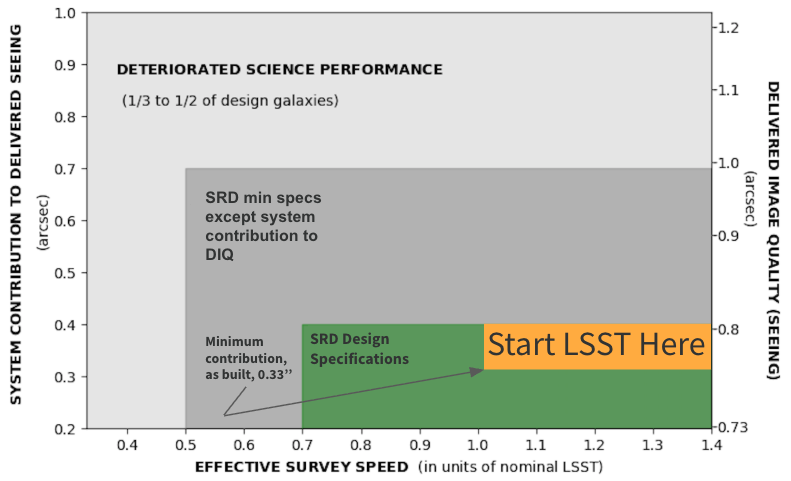
\includegraphics[width=0.85\linewidth]{speed3.png}
\caption{Image quality versus effective survey speed or Normalized \'{E}tendue. The large orange rectangle represents the region in this space within which we can confidently start the LSST while working to maintain and improve performance.}
\label{speed3}
\end{figure}

\subsection{Normalized \'{E}tendue}
Much of the effective speed (Normalized  \'{E}tendue) is already demonstrated to be sufficient to start the LSST, The field of view factor, fA, is excellent and stable. The sensitivity factor, fS, is also very good. This factor has the potential to help overall performance because of its dependence on delivered image quality. Getting the system contribution from 0.6 to 0.4 (coupled with site free air atmospheric seeing of 0.7$\arcsec$) would raise fS from 0.94 to 1.3. Apart from this, all the optics are delivered as is the focal plane. The performance of all these components is excellent and can be maintained. The observing efficiency or fO is also in good shape. The telescope dynamic performance (slew speed, acceleration, and jerk) is sufficient for the LSST planned cadence. 

The TMA is capable of accelerating more than we currently operate it. Higher acceleration requires improvements in the control of dynamic loads on the M1M3 glass via force actuators. However the current performance with glass is captured in the scheduler simulator and is only a modest hit to overall survey speed. We will continue to work on improved dynamic control even as we operate for LSST. Slew and settle performance are well understood and adequate. Modest gains on fO are forecast for the rest of SV and early operations. We expect the current value to go from 0.97 to 1.05. 

This leaves the System Availability, Current performance of 0.75 needs to be improved. Doing only science like observations we have reached 85$\%$ at times. We need to continue to improve on procedures and reliability of systems throughout the summit facility as we go forward. This means training for faster troubleshooting and fault recovery, making communications on the telescope system bus more reliable, improving reliability of telescope, dome, and camera functions. These have all seen marked progress as expected thoughout system integration, test, and commissioning. We will assume current performance of 75$\%$ conservatively. 

Using the combined SRD minimum specifications the lowest Normalized \'{E}tendue allowed is 0.7. This level is nearly in hand; see Table~\ref{tab:factors} and the ''Sustained Performance values''. We will start the LSST consistent with System Availability of 75$\%$ which leads to fE \~1.0 using the Demonstrated Capability column f factors in Table~\ref{tab:factors}. However, the actual value will be better given that we expect the System Availability to improve significantly. 

\newpage
